\documentclass[12pt]{article}
\usepackage[margin=0.5in]{geometry}
\usepackage{amsmath}
\usepackage{amssymb}
\usepackage{graphicx}
\usepackage{silence}
\WarningsOff[latex]
\usepackage{float}
\graphicspath{ {./pics/} }
\linespread{1.2}
\newcommand{\code}{\texttt}
\usepackage{csquotes}

\begin{document}
\subsection*{Q1.}
Since we use simple uniform hashing, the average number of elements that hash to the same array would be \(\alpha = \frac{n}{m}\), where \(n\) is the total number of elements in the hash table, and \(m\) is the number of slots.

\paragraph{(a).} Given that we use sorted arrays as the chaining components for the hash table:\\ On average, the time complexity for search would be \(O(1+\log(\alpha))\),  Here, \(O(1)\) is the time taken to compute \(h(k)\), and \(O(\log(\alpha))\) is the time to search for the key inside the array at slot \(h(k)\). We achieve logarithmic runtime as we could perform binary search on the sorted array, since arrays allow random access. However, if \(\alpha\) is very small, we would not have much benefit from the usual way of using linked list as the chaining component (runtime being \(O(1+\alpha)\)). But in the case that \(n \gg m\), then the runtime would improve.

\paragraph{(b).} Given that we need to run a merge sort every time we insert an element:\\
On average, the time complexity for insertion would be \(O(1+\alpha\log(\alpha))\), where \(O(1)\) is the time to compute \(h(k)\), and \(O(\alpha\log(\alpha))\) is the time to perform the merge sort on the array at slot \(h(k)\). If we do not keep track of the current number of elements in the array, then we also have an additional cost of \(O(\alpha)\) to search to the end for an empty spot, otherwise it would just take \(O(1)\) time to append. Yet in the end, the insertion time would be worse than the original scheme of using linked lists, as it only costs \(O(1)\) time to add the key to the front of the linked list.

\paragraph{(c).} Deletion with sorted arrays would remain the same as using linked lists, i.e. \(O(1 +\alpha)\). \(O(1)\) is the time to compute \(h(k)\), and \(O(\alpha)\) is the total cost for deletion. To delete, we first need to search for the key, so it takes \(O(\log(\alpha))\) to perform binary search, then \(O(1)\) to remove the key, and at the end, we need to fill in the empty space by shifting all elements greater than the deleted key one slot to the left. In the worst case, the deleted key is the first element, so we need to shift all remaining elements, which is \(O(\alpha)\). Since \(O(\log(\alpha)) \in O(\alpha)\), we have the overall cost for search-delete-shift as \(O(\alpha)\). With linked lists, deletion is also \(O(\alpha)\). We need to traverse the list to search for the previous element of the target, then change its pointer to the next (\(O(1)\)), and free memory for the target(\(O(1)\)). In the worst case, the target is the last element, so we require \(O(\alpha)\).

\subsection*{Q2.}
His claim is not correct for all situations. There is no guarantee that the leaves of a complete binary tree are on the same level. There could be missing right-most nodes on the last level. As illustrated in Figure 1, all internal nodes of a complete binary tree have two children, but the leaves here are not on the same level, meaning that if we color all nodes as black, the number of black nodes from root to a leaf is not the same for all paths. This violates the red black tree property:
\begin{displayquote}[][]
     For each node, all paths from this node to each of its leaves contain the same number of black nodes.
\end{displayquote}
Hence, it is not a red black tree in this case.
\begin{figure}[H]
     \centering
     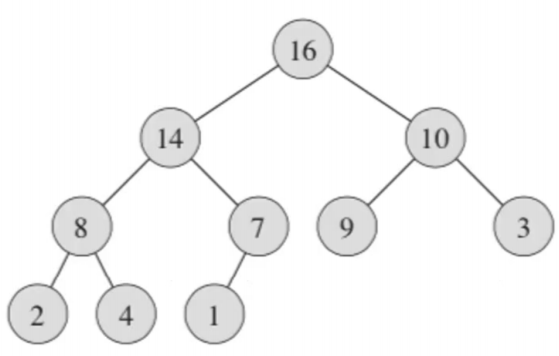
\includegraphics[scale =0.8]{q2a.png} 
     \caption{missing right-most nodes}
\end{figure}

\noindent However, if we have a perfect binary tree, which is a complete binary tree with all leaves on the same level (assuming leaves are nil), then it is valid red black tree:
     \begin{enumerate}
          \setlength \itemsep{0em} 
          \item the root is black
          \item leaves are black nils
          \item there is no consecutive red nodes along any path since there are no red nodes at all
          \item all paths from a node to its leaves contain the same number of black nodes.
     \end{enumerate}

\subsection*{Q3.}
An avl tree is a self balancing binary search tree that has the property that, for any node \(x\) in the tree, \(x\) has at most two children, and \(x.left.key \leq x.key \leq x.right.key\). Although for an avl tree, we might need rotation for insertion and deletion operations in order to maintain the balance factor, we still guarantee that the bst property holds. So the node with the minimum key is the left-most node in the tree. We could find it by traversing down the tree from the root, and always choosing the left subtree to traverse, until we find the left subtree to be nil, then the current node contains the minimum key. Similarly, the node with the maximum key is the right-most node in the tree. Beginning from the root, we always traverse the right subtree, until the right subtree is nil, then the current node contains the maximum key. 

\subsection*{Q5.}
\paragraph{(a).}
\textbf{Sub-problems:} We use slightly different sub-problems. We find the longest strictly decreasing sequence(LDS) of the prefixes of the original sequence, where the LDS is ended with the last element(box size) of the prefix. We also find the length of such LDS. The solution to the original problem would be the longest sequence among all solutions to the sub-problems.\\
\textbf{Relation between sub-problems:}
\begin{itemize}
     \setlength \itemsep{0em} 
     \item On LDS:\\
     Suppose \(P_i = [(r_1,h_1), (r_2, h_2), \hdots, (r_i, h_i)]\) is the input sequence, then a LDS of \(P_i\) which ends with the element \((r_i, h_i)\), denoted as LDS(\(P_i\)), is a longest sequence among \(S_k\) for \textbf{all} \(k \in [1, i-1]\) where
     \begin{equation*}
          S_k = 
          \begin{cases}
               \text{LDS(\(P_k\))} + [(r_i, h_i)] & \text{if } r_k > r_i \text{ and } h_k > h_i \\
               [(r_i, h_i)] & \text{if } r_k \leq r_i \text{ or } h_k \leq h_i
          \end{cases}
     \end{equation*}
     Here \('+'\) means concatenation of two sequences, and \(P_k\) is the sequence \([(r_1,h_1), (r_2, h_2), \hdots, (r_k, h_k)]\).
     \begin{itemize}
          \item LDS of \(P_k\) for some k
          \item \([(r_i, h_i)]\) if for all \(k \in [1, i-1]\) \(r_k \leq r_i \text{ or } h_k \leq h_i\)
     \end{itemize}
     \item On the length of LDS:
\end{itemize}
 


\end{document}